\chapter{Further development}
\label{chapter:further}

The objective of this chapter is to describe how the team envisions further development of the system. The envisioned architecture is show in figure~\ref{fig:idealArchitecture}. This includes both unfinished functionality and the concepts the team were unable to implement because of technical restrictions or time constraints.

Firstly, we will examine software improvements and how to improve Wattitude and implement the missing functionality. This involves functionality left out due to time constrictions, and features that need improvements. 

Then, all new concepts the team have discussed during the project, but not have implemented in to the app are discussed. This includes how the team envisions functionality for measuring power production and methods for including gamification into the app. 

Lastly, some insight into hardware solutions needed to get live data from devices in your house will be provided. 

\begin{figure}[H]
\centering
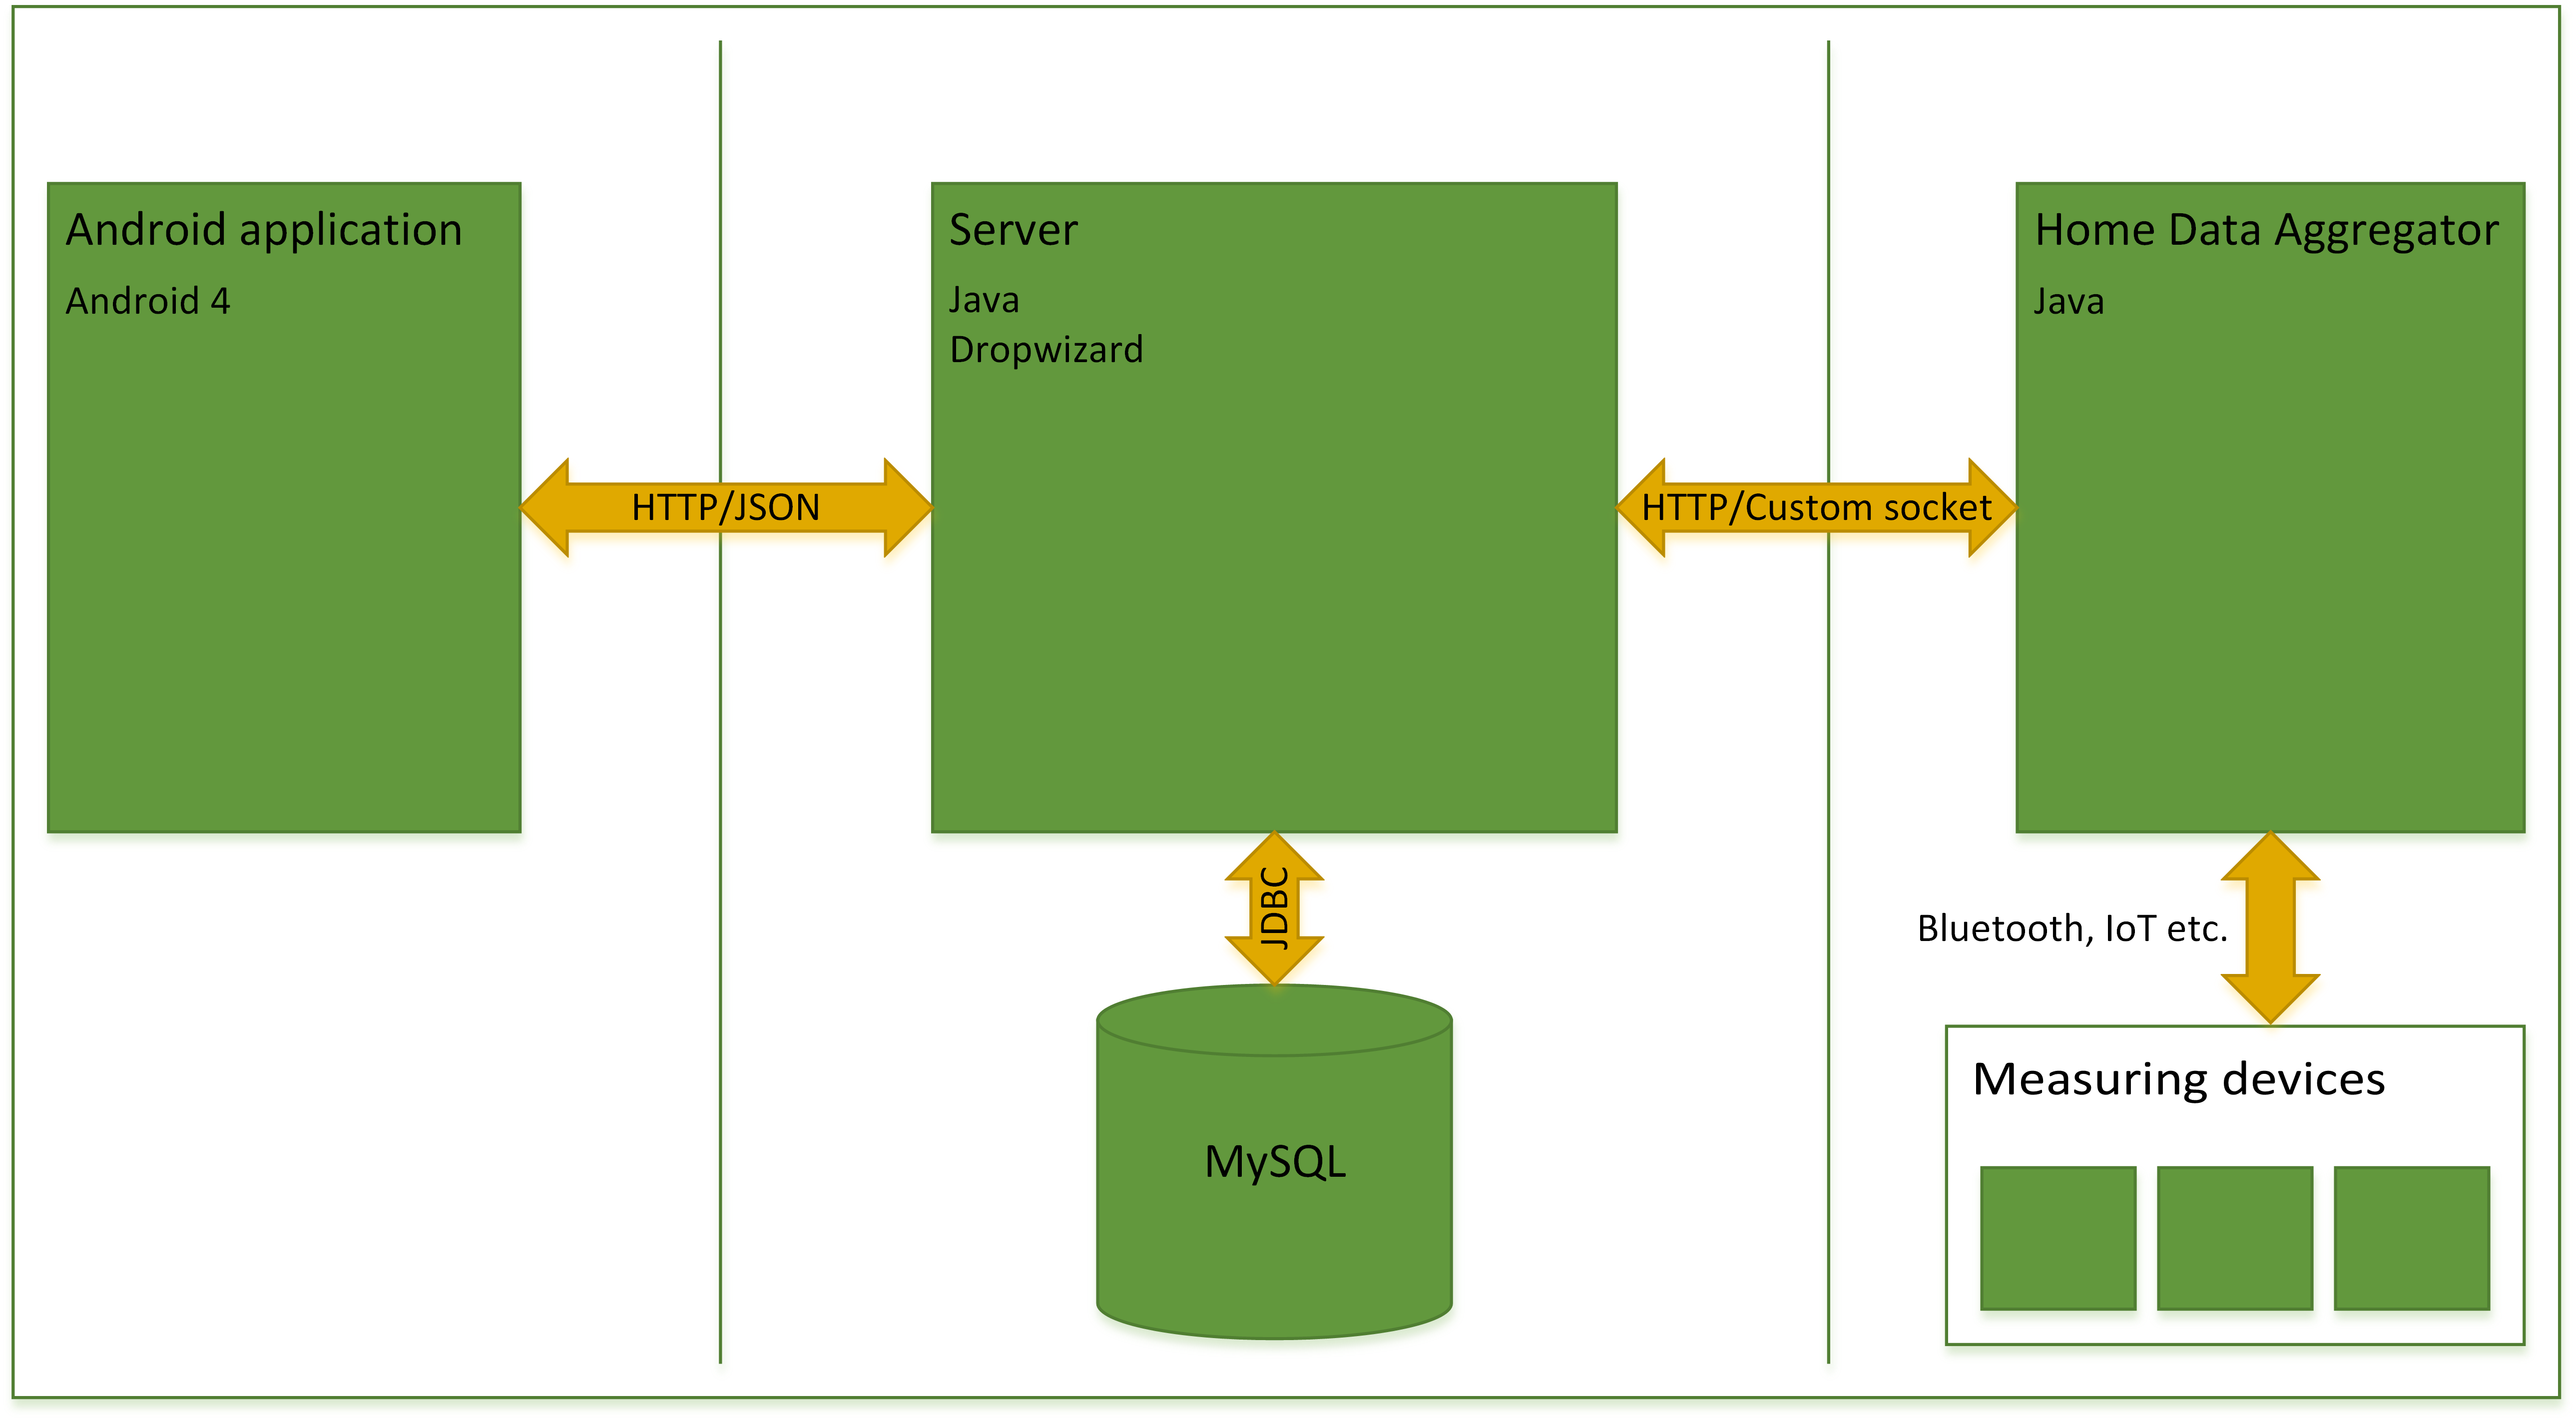
\includegraphics[height=0.3\textheight]{ch/further/fig/architecture.png}
\caption{Ideal Wattitude architecture.}
\label{fig:idealArchitecture}
\end{figure}

\input ch/further/sec/improvements.tex
\input ch/further/sec/concepts.tex
\input ch/further/sec/hardware.tex